\documentclass[11pt]{article}

\usepackage[utf8]{inputenc}
\usepackage{acl2015}
%\usepackage{times}
\usepackage{url}
%\usepackage{latexsym}
\usepackage{natbib}
\usepackage{graphicx}
\usepackage{multicol}

\title{This Time With Feeling: Sentiment to ML Headlines}

\author{Ben Arnoldy \\
  University of California, Berkeley \\
  {\tt arnoldyb@berkeley.edu} \\\And
  Mark Paluta \\
  University of California, Berkeley \\
  {\tt mpaluta@berkeley.edu} \\}
  
\date{July 2019}

\begin{document}

\maketitle

\begin{abstract}
    
\end{abstract}

\section{Introduction}
The art of good headline generation is not as simple as summarizing relevant details; it requires wit, originality, and a tone that matches the piece. Algorithms have made improvements in summarization, but still struggle with these more nuanced elements. Despite this shortcoming, algorithms can still be useful to an editor, suggesting a number of possible headlines to provide inspiration or to refine. We propose an incremental improvement in automatic headline generation by incorporating tonal bias to match the underlying content.

\section{Background}
Headline generation is primarily studied as a summarization task. Current approaches to summarization involve an encoder-decoder architecture \citep{rush2015neural} with a ROUGE evaluation metric \cite{Ayana2017}. ROUGE is a recall-oriented metric to score a generated summary against a reference summary \cite{lin-2004-rouge}. Specific variants include ROUGE-N, scoring the number of common N-grams, and ROUGE-L, scoring the longest common subsequence. Recent refinements to headline generation include adversarial reward systems to combat repetition \cite{DBLP:journals/corr/abs-1902-07110} and applying state-of-the-art Transformer algorithms \cite{DBLP:journals/corr/abs-1901-07786}.

While most work on headline generation focuses exclusively on summarization, two recent papers in other summarization domains explored efforts to add desired sentiment. One naive approach pre-processed sentences in the body of the corpus to generate sentence-level sentiment scores and simply dropped those sentences that were mismatched from the desired polarity (positive or negative) \cite{DBLP:journals/corr/abs-1802-09426}. Another more elaborate approach for customer review summaries added a discriminator to evaluate the sentiment of generated summaries, looping back to the generator to optimize on this additional criterion \cite{DBLP:journals/corr/HuYLSX17}. 
\section{Methodology}
We propose building a Transformer algorithm along the lines of Gavrilov et al (4), but adding sentiment into the model in the spirit of () and (). Following Gavrilov(4), we will use an encoder-decoder architecture, Adam optimizer, and the set of specific hyperparameters outlined by Gavrilov(4) as our baseline. We will experiment with polarity functions to capture various types of sentiment. We will use the annotated Gigaword dataset. 
	To test the quality of the generated headlines, we will begin with the ROUGE metric (7). We will then employ a novel metric by combining ROUGE with the Mean Squared Error of the difference between the sentiment scores of the input document and generated headline. Our goal is to learn whether training with sentimentality in the loop improves overall results through better handling of sentimentality and tone.
\section{Experiments}
\subsection{Subsection template if needed}
\section{Conclusions}

\begin{figure}[h!]
\centering
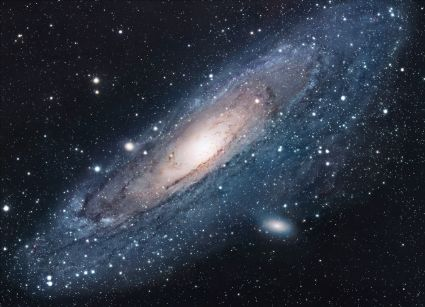
\includegraphics[scale=1.7]{universe}
\caption{The Universe}
\label{fig:universe}
\end{figure}

URL example
\url{http://acl2015.org/publication.html}.

"citing Rush here" \citep{rush2015neural}
"citing Ayana here" \cite{Ayana2017}
"citing Peng Xu here" \cite{DBLP:journals/corr/abs-1902-07110}
"citing Gavrilov here" \cite{DBLP:journals/corr/abs-1901-07786}
"citing Chaudari here" \cite{DBLP:journals/corr/abs-1802-09426}
"citing Zhiting Hu here" \cite{DBLP:journals/corr/HuYLSX17}
"citing Lin here" \cite{lin-2004-rouge}
"citing Attention is all you Need here" \cite{DBLP:journals/corr/VaswaniSPUJGKP17}

\bibliographystyle{plain}
\bibliography{references}
\end{document}




